\section{Modelagem Matemática}
\label{sec:modelagem-matematica}

A modelagem matemática da dinâmica do veículo é importante para o seu projeto. A partir dessa, é possível saber a força necessária no eixo X para se atingir o requisito de velocidade de dois metros por segundo. Por consequência, consegue-se selecionar um propulsor que consiga exercer essa força no veículo e a partir da escolha do propulsor, diversos componentes também podem ser especificados. Visto que o modelo matemático é o começo de toda essa cadeia de decisões de projeto, esse será o ponto de partida para as definições mais específicas do projeto. Adicionalmente, o modelo matemática influencia o controle e localização do veículo, pois pode ser utilizado para estimação de deslocamento e para otimização da lei de controle.

\subsection{Modelo Dinâmico do Veículo}

Existem diversos tipos de modelos matemáticos que podem ser adotados para a representação da dinâmica de um submarino \cite{Antonelli2018} \cite{fossen2011handbook}. A principal diferença entre cada tipo de modelo é quanto ao número de DOF a serem considerados, o grau de linearização e desacoplamento, e os fenômenos mecânicos do deslocamento de um corpo rígido na água a serem considerados. A fórmula geral para o modelo dinâmico de um veículo marinho \cite{fossen1994guidance} está representada na Equação \ref{eqn:marine_vehicle_model}, as quais tem parâmetros e funções que estão discriminadas na Tabela \ref{tab:eqn_param_description}. No modelo matemático, as linhas e colunas correspondem aos graus de liberdade na seguinte ordem: x, y, z, \textit{roll}, \textit{pitch} e \textit{yaw}. Ademais, a notação utilizada para modelagem do veículo está descrita em \cite{fossen2011handbook}, a qual corresponde a notação adotada pela SNAME (Sociedade Naval de Engenheiros e Arquitetos Marítimos).

\begin{equation}
	\label{eqn:marine_vehicle_model}
	M\dot{v} + C(v)v + D(v)v + g(\eta) + g_o = \tau + \tau_{e}
\end{equation}

\begin{table}
	\centering
	\label{tab:eqn_param_description}
	\caption{Tabela de descrição dos parâmetros da Equação \ref{eqn:marine_vehicle_model}}
	\begin{tabular}{ | c | c | } 
		\hline
		\textbf{Símbolo} & \textbf{Descrição}\\
		\hline
		$\eta$ & vetor de pose [6x1]\\ 
		\hline
		$v$ & vetor de velocidade [6x1]\\ 
		\hline
		$M$ & matriz de inércia [6x6]\\ 
		\hline
		$C$ & matriz coriolis em função da velocidade [6x6]\\ 
		\hline
		$D$ & matriz de amortecimento em função da velocidade [6x6]\\ 
		\hline
		$g$ & vetor de forças restauradoras hidrostáticas [6x1]\\ 
		\hline
		$g_o$ & vetor de força restauradoras por sistemas de lastro [6x1]\\ 
		\hline
		$\tau$ & vetor de força dos propulsores [6x1]\\ 
		\hline
		$\tau_e$ & vetor de forças externas de perturbação [6x1]\\ 
		\hline
	\end{tabular}
\end{table}

O sistema de referência do veículo é NED (\textit{North East Down}), isso significa que o sistemas de coordenadas do veículo tem o eixo x saindo do seu centro para a parte frontal, o eixo y saindo do seu centro para a esquerda e o z saindo do seu centro para baixo. Esse sistema foi adotado por convenção de veículos submarinos, na qual toda modelagem é baseada nesse sistema de coordenadas \cite{Antonelli2018} \cite{fossen2011handbook} \cite{fossen1994guidance}. Outra premissa a ser utilizada na modelagem é que o sistema de coordenadas é originado no centro de gravidade, de forma a facilitar a modelagem matemática. O veículo foi projetado para ser simétrico em relação aos planos XZ e YZ, além disso, quase todos os componentes são simétricos em relação aos seus plano XY. Essa premissa facilita o controle do veículo, visto que essas simetrias desacoplam o sistema, de forma que a movimentação do veículo em um grau de liberdade, não gera uma força em outra direção. Portanto, todos os componentes do modelo serão matrizes diagonais, pois o sistema é considerado desacoplado e pois os únicos termos que não relacionam um grau de liberdade com o outro é justamente a diagonal das matrizes.

Na Equação \ref{eqn:marine_vehicle_model} pode se observar sete termos sendo somados, porém alguns desses termos não serão considerados. Os termos $\tau_e$ e $g_o$ não serão considerados, pois o veículo não foi projetado com sistemas de lastros e porque perturbações no veículo não serão medidas ou consideradas em seu modelo. Ademais, o termo de coriolis também vai ser desconsiderado pois é a força gerada pela rotação da terra, a qual em pequenas velocidades é próxima a zero e não precisa ser considerada \cite{rov_modeling_1} \cite{rov_modeling_2}. Por fim, eliminando esses três componentes da equação, obtém-se a Equação \ref{eqn:marine_vehicle_model_short}  que vai ser utilizada.

\begin{equation}
	\label{eqn:marine_vehicle_model_short}
	M\dot{v} + D(v)v + g(\eta) = \tau 
\end{equation}

\subsection{Matriz de Inércia}

A matriz de inércia de um corpo rígido $M_{RB}$ tem o formato da Equação \ref{eqn:inertia_matrix}, porém no caso de um veículo submarino a matriz de inércia $M$ é representada pela Equação \ref{eqn:uw_inertia_matrix} \cite{fossen2011handbook}. O termo $M_A$ da é a matriz de massa adicional. A matriz de massa adicional, definida pela Equação \ref{eqn:added_mass_matrix} representa a força que o fluído no qual o veículo está imerso exerce no veículo durante o seu deslocamento. 

\begin{equation}
	\label{eqn:inertia_matrix}
	M_{RB} = 
	\begin{bmatrix}
		m & 0 & 0 & 0 & mz_g & -my_g\\
		0 & m & 0 & -mz_g & 0 & mx_g\\
		0 & 0 & m & my_g & -mx_g & 0\\
		0 & -mz_g & my_g & I_x & -I_{xy} & -I_{xz}\\
		mz_g & 0 & -mx_g & -I_{yx} & I_y & -I_{yz}\\
		-my_g & mx_g & 0 & -I_{zx} & -I_{zy} & I_z				
	\end{bmatrix}
\end{equation}

\begin{equation}
	\label{eqn:uw_inertia_matrix}
	M = M_A + M_{RB}
\end{equation}

\begin{equation}
	\label{eqn:added_mass_matrix}
	M_{A} = 
	\begin{bmatrix}
		X_{\dot{u}} & 0 & 0 & 0 & 0 & 0\\
		0 & Y_{\dot{v}} & 0 & 0 & 0 & 0\\
		0 & 0 & Z_{\dot{w}} & 0 & 0 & 0\\
		0 & 0 & 0 & K_{\dot{p}} & 0 & 0\\
		0 & 0 & 0 & 0 & M_{\dot{q}} & 0\\
		0 & 0 & 0 & 0 & 0 & N_{\dot{r}} 
	\end{bmatrix}
\end{equation}

Os parâmetros da matriz de inércia do corpo rígido são definidos na Tabela  \ref{tab:inertia_matrix_params}. Esses parâmetros são comumente obtidos pelos \textit{software} de CAD, no caso se utilizou o mesmo software usado na modelagem, o \textit{OnShape}. Os parâmetros da matriz de massa adicional estão definidos na Tabela \ref{tab:added_mass_matrix_params}, para obtenção desses parâmetros se utilizou o \textit{software capytaine}, o qual é utilizado especificamente para estimação de parâmetros de estruturas e veículos marinhos a partir de um arquivo com o formato do que se quer estimar \cite{capytaine}.

\begin{table}[H]
	\centering
	\label{tab:inertia_matrix}
	\caption{Tabela de valores dos parâmetros da Equação \ref{eqn:inertia_matrix}}
	$\begin{array}{c c c}
		\begin{matrix} 
			I_x & 0.12915888 & kg m^{2}\\ 
			I_y & 0.27890934 & kg m^{2}\\ `
			I_z & 0.33540447 & kg m^{2}\\ 
			I_{xy} & 0 & kg m^{2}\\
			I_{xz} & 0 & kg m^{2}\\
			I_{yz} & 0 & kg m^{2}\\
			m & 9.19851484 & kg\\ 
			x_g & 0 & m\\ 
			y_g & 0 & m\\ 
			z_g & 0 & m
		\end{matrix}
	\end{array}$
\end{table}

\begin{table}[H]
	\centering
	\label{tab:added_mass_matrix_params}
	\caption{Tabela de valores dos parâmetros da Equação \ref{eqn:added_mass_matrix}}
	$\begin{array}{c c c}
		\begin{matrix} 
			X_{\dot{u}} & 6.4832996 & kg m^{2}\\ 
			Y_{\dot{v}} & 10.271688 & kg m^{2}\\ 
			Z_{\dot{w}} & 47.014015 & kg m^{2}\\ 
			K_{\dot{p}} & 0.1089654 & kg m^{2}\\
			M_{\dot{q}} & 0.0962604 & kg m^{2}\\
			N_{\dot{r}} & 0.1505059 & kg m^{2}
		\end{matrix}
	\end{array}$
\end{table}

\subsection{Forças de Propulsão}

As forças de propulsão, representadas pela Equação \ref{eqn:propulsion_force}, são as forças em cada grau de liberdade gerada por cada motor. Na Equação \ref{eqn:propulsion_force}, a matriz $B$ representa a relação geométrica do vetor de direção da força de cada propulsor com os seis graus de liberdade, na qual cada linha um dos graus de liberdade e cada coluna representa um propulsor do veículo, os quais foram numerados de acordo com a Figura \ref{fig:propellers}. Na matriz existem termos que não foram apresentados, esses estão descritos na Tabela \ref{tab:aux_terms_desc} e nas Equações \ref{eqn:aux_terms_eqn}.

\begin{equation}
	\label{eqn:propulsion_force}
	\tau = Bu 
\end{equation}

\begin{equation}
	\label{eqn:b_matrix}
	B =
	\begin{bmatrix}
		0 & 0 & cos(\alpha_3) & cos(\alpha_4) & -cos(\alpha_5) & -cos(\alpha_6)\\
		0 & 0 & -sen(\alpha_3) & sen(\alpha_4) & -sen(\alpha_5) & sen(\alpha_6)\\
		1 & 1 & 0 & 0 & 0 & 0\\
		y_1 & y_2 & 0 & 0 & 0 & 0\\
		x_1 & x_2 & 0 & 0 & 0 & 0\\
		0 & 0 & d_3sen(\gamma_3) & -d_4sen(\gamma_4) & -d_5sen(\gamma_5) & d_6sen(\gamma_6) 
	\end{bmatrix}  
\end{equation}

\begin{figure}[H]
	\centering
	\caption{Propulsores do veículo}
	\label{fig:propellers}
	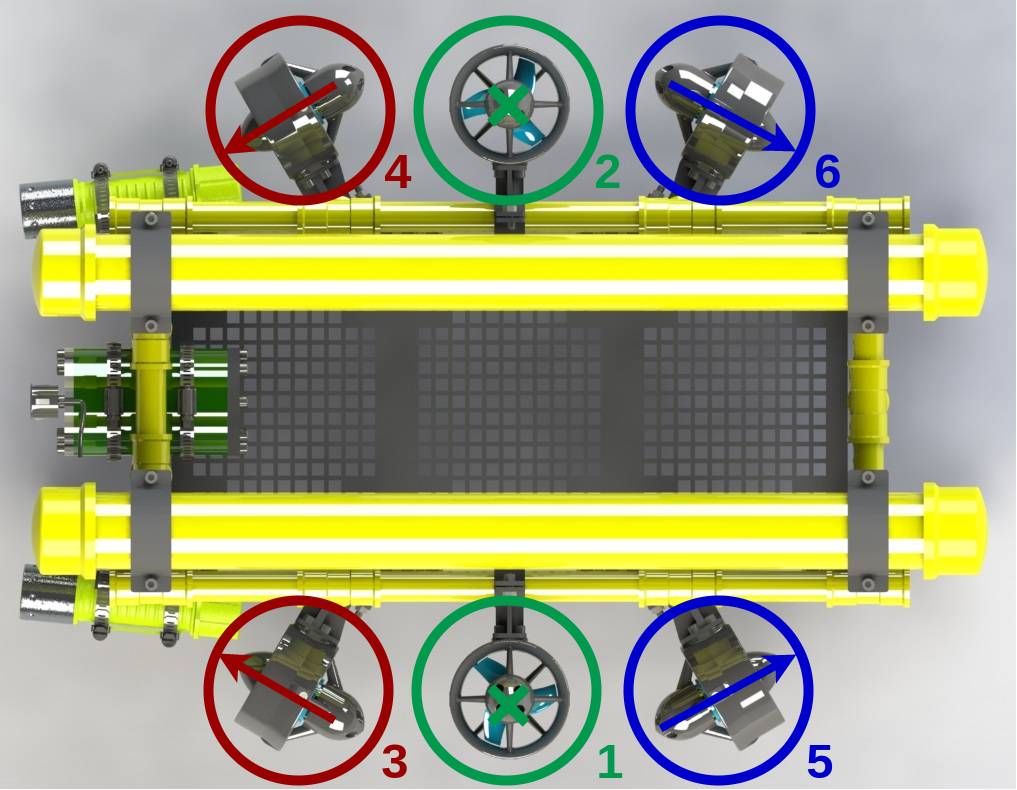
\includegraphics[width=0.8\linewidth]{images/brov_propulsion.png}\\
	\footnotesize Fonte: Autores
\end{figure}

\begin{table}[H]
	\centering
	\label{tab:aux_terms_desc}
	\caption{Tabela de descrição dos parâmetros da Equação \ref{eqn:b_matrix}}
	\begin{tabular}{ | c | c | } 
		\hline
		\textbf{Símbolo} & \textbf{Descrição}\\
		\hline
		$\alpha_n $ & módulo do ângulo entre eixo do motor com eixo x do veículo\\ 
		\hline
		$x_n, y_n, z_n $ & coordenadas dos motores em relação a posição de referência (CoG) \\ 
		\hline
		$d_n$ & distância do motor para o CoG no plano XY\\ 
		\hline
		$\gamma_n$ & soma de $\alpha$ e $\varphi$\\ 
		\hline
		$\varphi_n$ &  ângulo entre eixo x do veículo e reta que parte do CoG \\  & para o motor no plano XY \\
		\hline
	\end{tabular}
\end{table}

\begin{equation}
	\label{eqn:aux_terms_eqn}
	\begin{aligned} 
		\alpha_n = 30^{\circ} \\
		d_n = \sqrt{x_n^{2} + y_n^{2}} \\
		\gamma_n = \varphi_n + \alpha_n \\
		\varphi_n = tan^{-1}(\frac{y_n}{x_n}) 
	\end{aligned}
\end{equation}

\begin{figure}[H]
	\centering
	\caption{Visualização de parâmetros da matriz da Equação \ref{eqn:b_matrix} em vista superior de representação do veículo. }
	\label{fig:side_thrusters}
	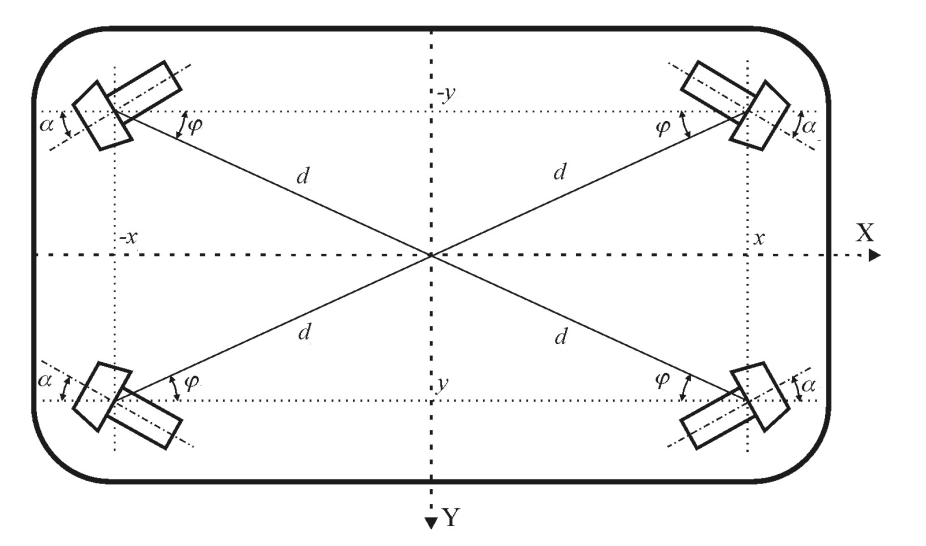
\includegraphics[width=0.8\linewidth]{images/side_thrusters.png}\\
	\footnotesize Fonte: Adaptada de \cite{thruster_allocation}
\end{figure}

A obtenção da matriz da Equação \ref{eqn:b_matrix} é realizada através do cálculo das projeções dos vetores de força dos propulsores em cada grau de liberdade da movimentação do veículo. Para isso, os trabalhos \cite{Antonelli2018} \cite{fossen1994guidance} \cite{fossen2011handbook} \cite{rov_modeling_1}, \cite{rov_modeling_2} e principalmente \cite{thruster_allocation} foram utilizados como guias. Os parâmetros da matriz são medidas geométricas que também foram obtidas com o \textit{software} CAD de modelagem do veículo, seus valores estão na Tabela \ref{tab:b_matrix_param_values}. 

\begin{table}[H]
	\centering`
	\label{tab:b_matrix_param_values}
	\caption{Tabela de valores dos parâmetros da Equação \ref{eqn:b_matrix}}
	$\begin{array}{c c c}
		\begin{matrix} 
			x_1 & -0.0277 & m\\ 
			y_1 &  0.1932 & m\\ 
			x_2 & -0.0277 & m\\ 
			y_2 & -0.1932 & m\\ 
			\alpha_n & 30 & ^{\circ}\\		
			d_3 & 0.2188 & m\\ 		
			d_4 & 0.2188 & m\\ 		
			d_5 & 0.2519 & m\\ 		
			d_6 & 0.2519 & m\\ 
			\varphi_3 & 88.9221 & ^{\circ} \\
			\varphi_4 & 88.9221 & ^{\circ} \\
			\varphi_5 & 78.0432 & ^{\circ} \\
			\varphi_6 & 78.0432 & ^{\circ} 
		\end{matrix}
	\end{array}$
\end{table}

Dessa forma, se conclui a modelagem da força de propulsão do veículo. A partir dessa matriz é possível saber como acionar cada propulsor para se obter uma determinada força em um grau de liberdade do veículo, assim como saber qual a consequência dos acionamentos dos motores para o algoritmo de localização.

\subsection{Forças Restauradoras}

As forças restauradoras, representadas pela Equação \ref{eqn:restoring_force} \cite{rov_modeling_1}, são forças resultantes da atuação do empuxo no centro de flutuabilidade do pedo no centro de gravidade do veículo, que se comporta como um corpo rígido imerso em um fluído. A descrição dos parâmetros da Equação \ref{eqn:restoring_force} pode ser observada na Tabela \ref{tab:restoring_force_param_desc}.

\begin{equation}
	\label{eqn:restoring_force}
	g(\eta) =
	\begin{bmatrix}
		-(W-B)sen(\theta)\\
		(W-B)cos(\theta)sen(\phi)\\
		(W-B)cos(\theta)cos(\phi)\\
		(y_gW-y_bB)cos(\theta)cos(\phi) - (z_gW-z_bB)cos(\theta)sen(\phi)\\		
		(z_gW-z_bB)sen(\theta) - (x_gW-x_bB)cos(\theta)cos(\phi)\\
		(x_gW-x_bB)cos(\theta)sen(\phi) + (y_gW-y_bB)sen(\theta)
	\end{bmatrix}  
\end{equation}

\begin{table}[H]
	\centering
	\label{tab:restoring_force_param_desc}
	\caption{Tabela de descrição dos parâmetros e variáveis da Equação \ref{eqn:restoring_force}}
	\begin{tabular}{ | c | c | } 
		\hline
		\textbf{Símbolo} & \textbf{Descrição}\\
		\hline
		$W$ & Módulo da força peso\\ 
		\hline
		$B$ & Módulo da força empuxo\\ 
		\hline
		$\theta$ & ângulo \textit{yaw} do veículo\\ 
		\hline
		$\phi$ & ângulo \textit{roll} do veículo\\ 
		\hline
		$x_g, y_g, z_g $ & coordenadas do centro de gravidade em relação a posição de referência \\ 
		\hline
		$x_b, y_b, z_b $ & coordenadas do centro de flutuabilidade em relação a posição de referência\\ 
		\hline
	\end{tabular}
\end{table}

No início da desta seção algumas premissas de modelagem do veículo foram estabelecidas e justificadas. Uma dessas premissas consiste na adoção do CoG do veículo como posição de referência para sua modelagem, dessa forma, $x_g$, $y_g$ e $z_g$ são iguais a zero. Ademais, também definiu-se que o seria modelado para ser simétrico em relação aos planos XZ e YZ, dessa forma, o $x_b$ e $y_b$ ficaram muito próximos ao $x_g$ e $y_g$, portanto, também serão considerados iguais a zero. A partir disso, é possível simplificar a Equação \ref{eqn:restoring_force} na Equação \ref{eqn:restoring_force_short}, a qual tem parâmetros com valores detalhados na Tabela \ref{tab:restoring_force_param_value}. É importante observar que $\theta$ e $\phi$ são variáveis e por isso não tem seu valor definido.

\begin{equation}
	\label{eqn:restoring_force_short}
	g(\eta) =
	\begin{bmatrix}
		-(W-B)sen(\theta)\\
		(W-B)cos(\theta)sen(\phi)\\
		(W-B)cos(\theta)cos(\phi)\\
		z_bBcos(\theta)sen(\phi)\\		
		z_bBsen(\theta)\\
		0
	\end{bmatrix}  
\end{equation}

\begin{table}[H]
	\centering
	\label{tab:restoring_force_param_value}
	\caption{Tabela de valores dos parâmetros da Equação \ref{eqn:restoring_force_short}}
	$\begin{array}{c c c}
		\begin{matrix} 
			W & 90.1735 & \frac{kgm}{s^{2}} \\ 
			B &  92.3277 & \frac{kgm}{s^{2}} \\
			z_b &  -0.0164 & m
		\end{matrix}
	\end{array}$
\end{table}

É possível observar com a Tabela \ref{tab:restoring_force_param_value} que o peso é aproximadamente 2 Newtons menor do que o empuxo, logo, o veículo tem flutuabilidade positiva e somente é necessário 2 Newtons de força resultante dos propulsores para baixa para que o veículo afunde. Outra coisa importante de se observar é que o veículo naturalmente controla \textit{roll} e \textit{pitch}, visto que o termo 4 e 5 do vetor da Equação \ref{eqn:restoring_force_short} no intervalo de zero a $\frac{\pi}{2}$ é negativo e de $\frac{-\pi}{2}$ a zero é positivo, sempre levando esses ângulos pra zero.

\subsection{Força de Amortecimento}

A força de amortecimento ou arrasto, que é representada pela Equação \ref{eqn:damping}, é a força contraria ao movimento que é proporcional a velocidade do veículo. Na Equação \ref{eqn:damping}, $D_l$ representa uma matriz de coeficientes lineares do arrasto e $D_q$ uma matriz de coeficientes quadráticos do arrasto. De acordo com \cite{fossen2011handbook}, esse termo ocorre devido a 4 fenômenos, dos quais somente o derramamento de vórtices, representado pela Equação \ref{eqn:quadratic_damping}, tem grande influência e pode ser modelado fenomenologicamente. Os parâmetros da Equação \ref{eqn:quadratic_damping} tem sua descrição na Tabela \ref{tab:quadratic_damping_param_desc} e valores na Tabela \ref{tab:quadratic_damping_param_value}. 

\begin{equation}
	\label{eqn:damping}
	D = D_lv + D_qv^{2}
\end{equation}

\begin{equation}
	\label{eqn:quadratic_damping}
	D_q = -
	\begin{bmatrix}
		\frac{\rho C_dA_{fx}}{2} & 0 & 0 & 0 & 0 & 0\\
		0 & \frac{\rho C_dA_{fy}}{2} & 0 & 0 & 0 & 0\\
		0 & 0 & \frac{\rho C_dA_{fz}}{2} & 0 & 0 & 0\\
		0 & 0 & 0 & \frac{\rho C_dA_{fz}}{2} & 0 & 0\\
		0 & 0 & 0 & 0 & \frac{\rho C_dA_{fz}}{2} & 0\\
		0 & 0 & 0 & 0 & 0 & \frac{\rho C_dA_{fy}}{2} 
	\end{bmatrix}
\end{equation}

\begin{table}[H]
	\centering
	\label{tab:quadratic_damping_param_desc}
	\caption{Tabela de descrição dos parâmetros e variáveis da Equação \ref{eqn:quadratic_damping}}
	\begin{tabular}{ | c | c | } 
		\hline
		\textbf{Símbolo} & \textbf{Descrição}\\
		\hline
		$C_d$ & coeficiente de arrasto\\ 
		\hline
		$\rho$ & densidade do meio\\ 
		\hline
		$A_{nf}$ & área projetada no eixo n\\ 
		\hline
	\end{tabular}
\end{table}

\begin{table}[H]
	\centering
	\label{tab:quadratic_damping_param_value}
	\caption{Tabela de valores dos parâmetros da Equação \ref{eqn:quadratic_damping}}
	$\begin{array}{c c c}
		\begin{matrix} 
			\rho & 1023 & \frac{kg}{m^{3}} \\ 
			C_d &  1.17 & Admensional \\
			A_{xf} & 0.04705 & m² \\
			A_{yf} & 0.08222 & m² \\
			A_{zf} & 0.115115 & m² 
		\end{matrix}
	\end{array}$
\end{table}


%\begin{equation}
%	D_q = Bu_{max}
%\end{equation}
%
%\begin{equation}
%	\begin{matrix} 
%		v_{x} & 1.9956 & \frac{m}{s} \\
%		v_{y} & 1.1471 & \frac{m}{s} \\
%		v_{z} & 0.9694 & \frac{m}{s} \\
%		v_{yaw} & 5.5707 & \frac{^{\circ}}{s}
%	\end{matrix}
%\end{equation}